\chapter{\textit{Python}}

\section{Sejarah \textit{Python}}
Python merupakan bahasa pemrograman tingkat tinggi yang dapat digunakan banyak hal, \textit{Python} awalnya dirancang oleh \textbf{Guido van Rossum} pada tahun 1980 yang mana nama \textit{Python} sebelum sebesar sekarang yaitu \textit{ABC Programming Language} yang dijalankan di sistem operasi bernama \textit{Amoeba Operating System}. Guido merasakan kehebatan dan kemampuan serta fitur yang berada pada bahasa pemrograman ABC ini sehingga Guido mengambil siktaks-sintaks yang berada pada bahasa pemrograman ABC ini, tentu saja banyak komplain yang berdatangan sehingga Guido terus melakukan perbaikan pada bahasa pemrograman yang sedang ia buat kala itu. Lalu, disinilah nama \textit{Python} muncul dimuka bumi sebagai bahasa pemrograman, disaat Guido sedang menonton televisi dan menemukan kata '\textit{Monty Python's Flying Circus}'.

Bahasa \textit{Python} secara resmi dirilis pada tahun 1991, saat rilis pertama kali semua orang terkejut dengan sintaks yang dimiliki oleh \textit{Python} ketika dibandingkan dengan bahasa lain seperti \textit{Java, C, C++}, dan lain-lain pengekspresian bahasa ini cukup sederhana. Tujuan dari dibuatnya bahasa pemrograman ini adalah untuk mempermudah dalam membaca sebuah kode dari penulisan sintaks dan produktivitas dalam hal pengembangan tingkat lanjut.

\section{Perbedaan \textit{Python 2.x} dan \textit{Python 3.x}}
Banyak perbedaan yang akan kita temui jika kita dahulu pernah menggunakan \textit{python} versi 2.x cukup lama sehingga berpindah ke versi 3.x, berikut contoh perbedaan pada \textit{python} versi 2.x dan 3.x yang sangat penting untuk diketahui:

\begin{enumerate}

\item Perintah \textbf{print}
Perbedaan perintah \textit{print} pada dua versi ini adalah python 2.x tidak memakai kurung dan 3.x memakai kurung untuk perintah \textit{print} bisa dilihat pada gambar ~\ref{print} dan \ref{printnano}

\begin{figure}[H]
\centering
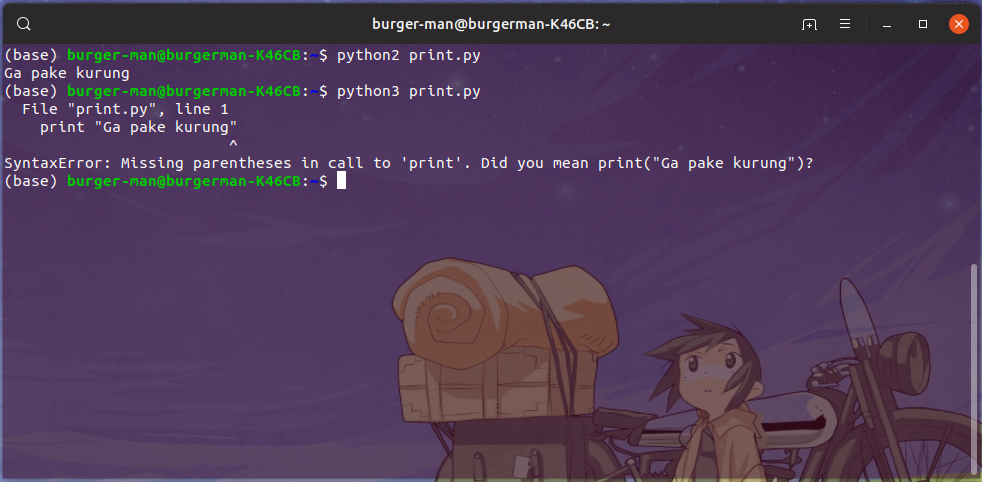
\includegraphics[width=1\textwidth]{figures/print.png}
\caption{Gambar hasil print}
\label{print}
\end{figure}

\begin{figure}[H]
\centering
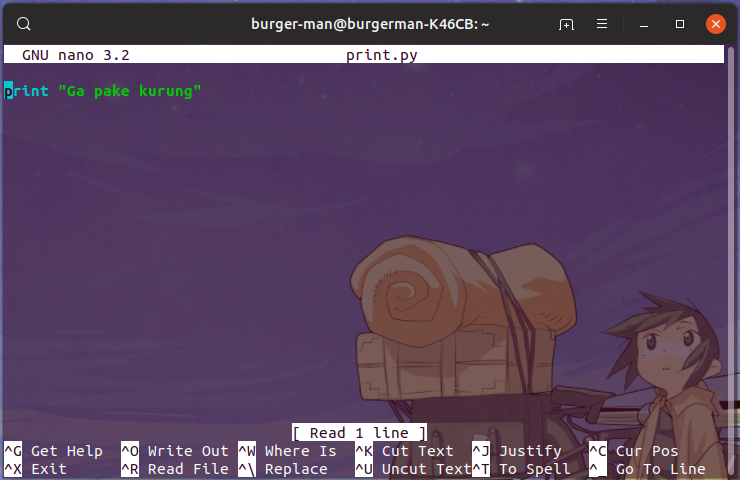
\includegraphics[width=1\textwidth]{figures/printnano.png}
\caption{Gambar perintah print}
\label{printnano}
\end{figure}

\item Perintah pembagian \textbf{\textit{integer}}
Hasil dari perintah pembagian cukup jelas berbeda yang mana versi 2.x tidak secara mendetail untuk hasilnya sehingga angka yang dihasilkan bilangan \textbf{\textit{integer}} sedangkan versi 3.x bertipe \textbf{\textit{float}} perbedaannya bisa dilihat pada gambar \ref{div} dan \ref{divnano}.

\begin{figure}[H]
\centering
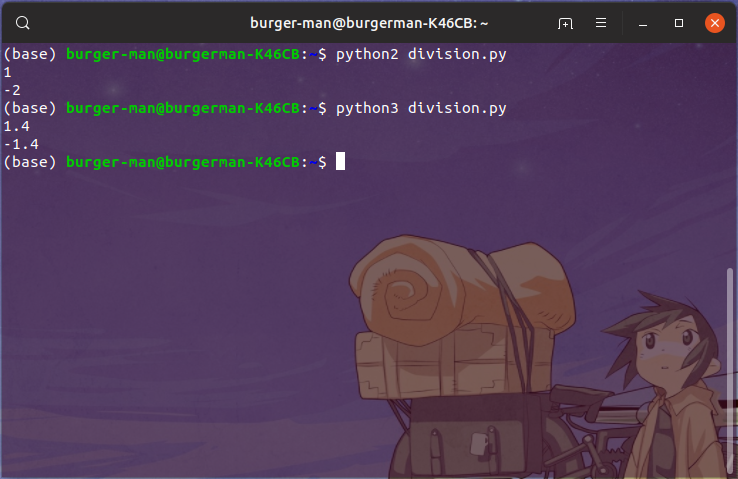
\includegraphics[width=1\textwidth]{figures/div.png}
\caption{Gambar hasil pembagian}
\label{div}
\end{figure}

\begin{figure}[H]
\centering
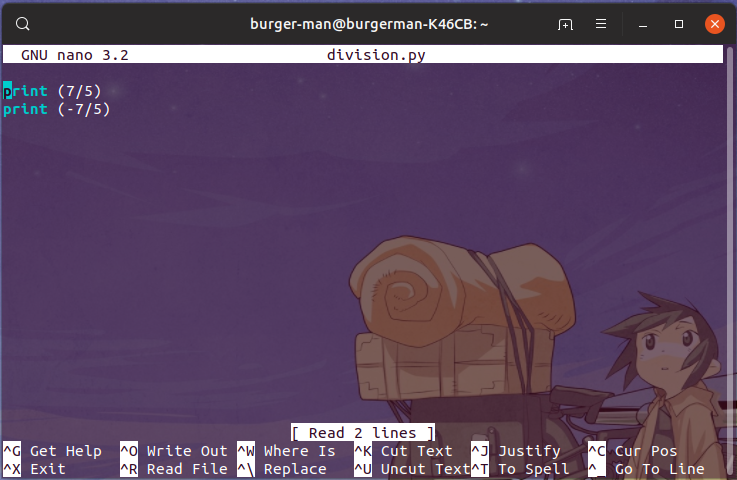
\includegraphics[width=1\textwidth]{figures/divnano.png}
\caption{Gambar perintah pembagian}
\label{divnano}
\end{figure}

\item \textit{\textbf{Try and Except}}
Perbedaan pada \textit{try and expcept} hanya berbeda di penggunaan \textbf{,} untuk versi 2.x dan \textbf{as} untuk versi 3.x.

\begin{figure}[H]
\centering
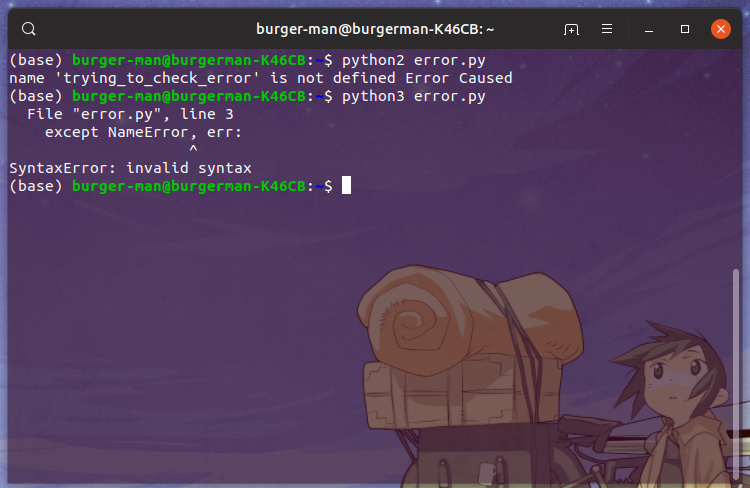
\includegraphics[width=1\textwidth]{figures/error.png}
\caption{Gambar hasil error}
\label{error}
\end{figure}

\begin{figure}[H]
\centering
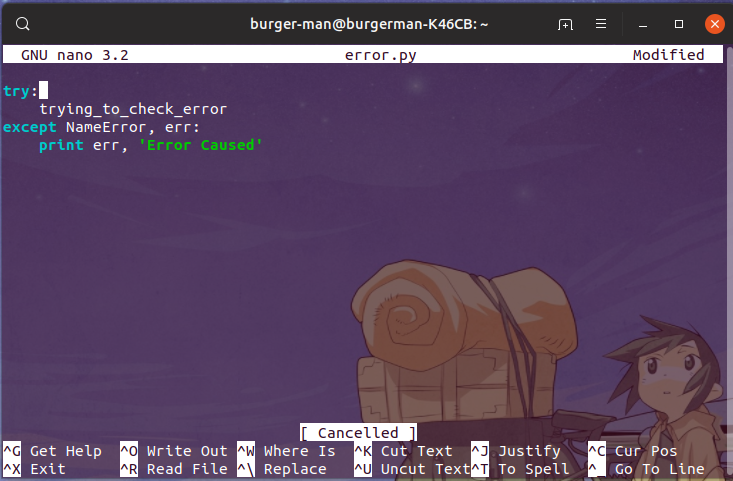
\includegraphics[width=1\textwidth]{figures/errornano.png}
\caption{Gambar perintah error}
\label{errornano}
\end{figure}

\item \textbf{\textit{Looping}}
Perbedaan pada looping hanya saja versi 3.x tidak bisa menggunakan sintaks \textbf{\textit{xrange}} lagi.

\begin{figure}[H]
\centering
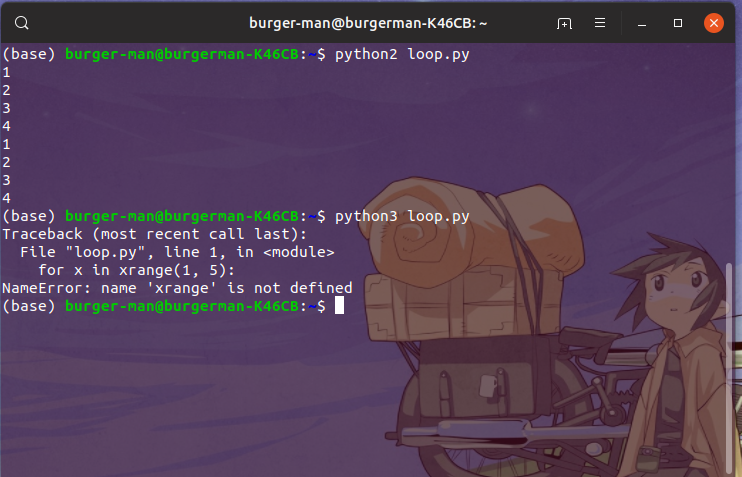
\includegraphics[width=1\textwidth]{figures/loop.png}
\caption{Gambar hasil looping}
\label{loop}
\end{figure}

\begin{figure}[H]
\centering
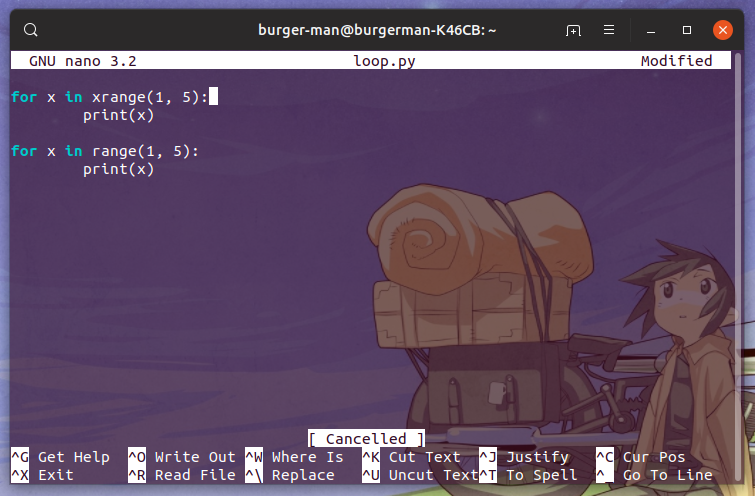
\includegraphics[width=1\textwidth]{figures/loopnano.png}
\caption{Gambar perintah looping}
\label{loopnano}
\end{figure}

\item \textbf{\textit{Unicode}}
Unicode ini cukup penting karena kita mengetahui bagaimana setiap versi merespons setiap unicode yang diberikan.

\begin{figure}[H]
\centering
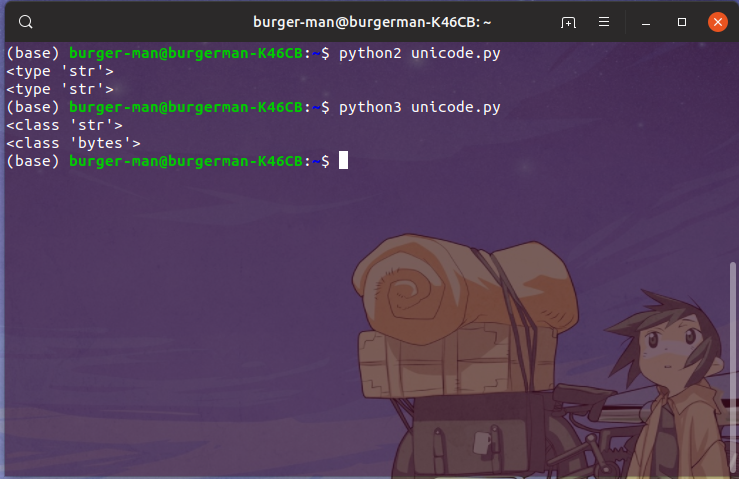
\includegraphics[width=1\textwidth]{figures/unicodebytes.png}
\caption{Gambar hasil unicode (bytes)}
\label{unibytes}
\end{figure}

\begin{figure}[H]
\centering
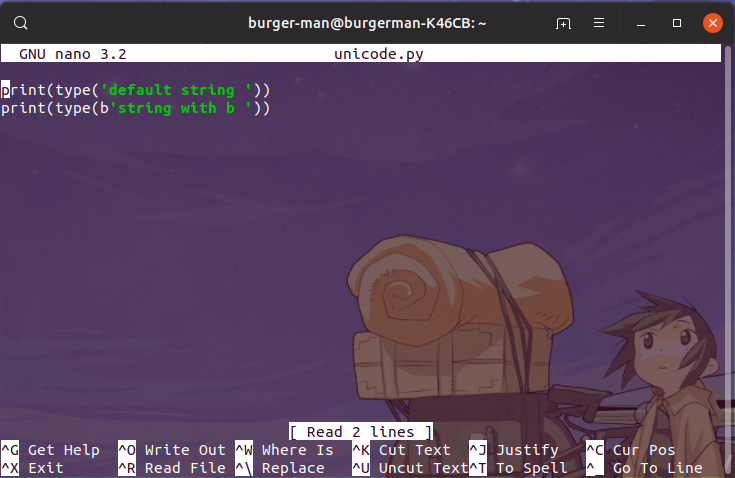
\includegraphics[width=1\textwidth]{figures/unicodebytesnano.png}
\caption{Gambar perintah unicode (bytes)}
\label{unibytesnano}
\end{figure}
Pada gambar ~\ref{unibytes} terlihat jelas bahwa perintah \textbf{\textit{bytes}} hanya direspon pada versi 3.x sedangkan versi 2.x merespon \textbf{\textit{string}}

\begin{figure}[H]
\centering
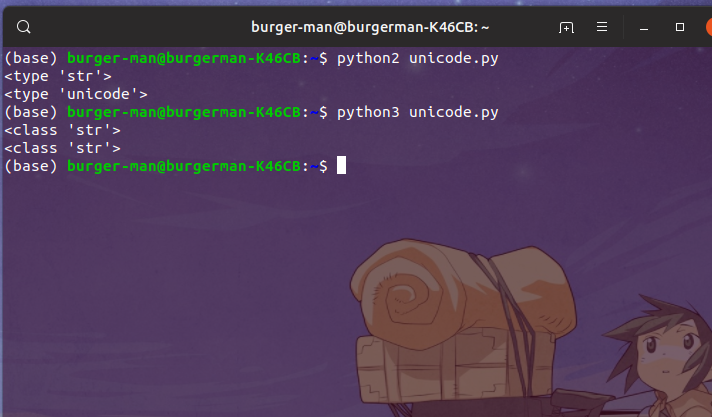
\includegraphics[width=1\textwidth]{figures/unicodeuni.png}
\caption{Gambar hasil unicode}
\label{unicodeuni}
\end{figure}

\begin{figure}[H]
\centering
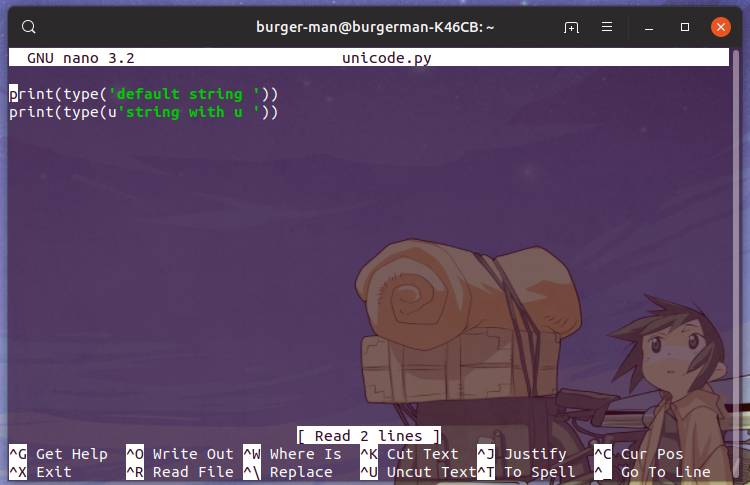
\includegraphics[width=1\textwidth]{figures/unicodeuninano.png}
\caption{Gambar perintah unicode}
\label{unicodeuninano}
\end{figure}

\end{enumerate}

\section{Installasi Python}
Untuk installasi kali ini akan bagi menjadi dua sistem operasi yaitu Windows (Windows 10), dan Linux (Ubuntu 19.04). Installasi menggunakan \textit{environtment} Anaconda sebagai installasi \textit{python}. Anaconda merupakan \textit{environment open-source} untuk bahasa pemrograman \textit{Python}, dan \textit{R} berfungsi untuk memanajemen penggunaan \textit{package} pada \textit{python} dan \textit{R}.

\subsection{Windows (Windows 10)}
Hal yang harus diperhatikan sebelum melakukan instalasi \textit{Anaconda Python}
\begin{enumerate}
 \item Perhatikan versi dari sistem operasi yang digunakan (versi 32bit atau 64bit)
 \item Download file anaconda yang sesuai dengan versi sistem operasi (32bit atau 64bit)
 \item \textit{Download Anaconda Python} https://www.anaconda.com/distribution/
\end{enumerate}

Berikut langkah-langkah instalasi anaconda.
\begin{enumerate}
\item Buka aplikasi \textit{installer Anaconda} tersebut lalu akan muncul  gambar \textit{installer anaconda}.
\begin{figure}[H]
        \centerline{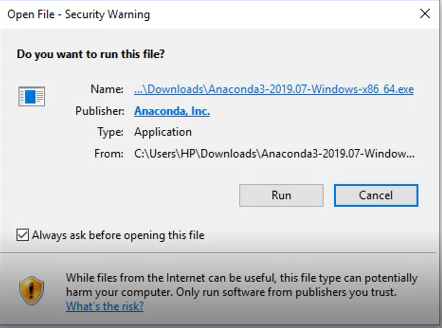
\includegraphics[scale=0.5]{figures/1}}
        \caption{Run Setup Anaconda}
		\label{langkah1}
\end{figure}

\item Tunggu hingga \textit{setup loading} selesai
\begin{figure}[H]
        \centerline{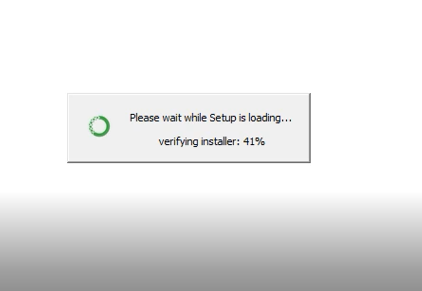
\includegraphics[scale=0.5]{figures/2}}
        \caption{Setup Loading}
		\label{langkah2}
\end{figure}


\item Jika \textit{setup loading} telah selesai, maka klik \textit{next}
\begin{figure}[H]
        \centerline{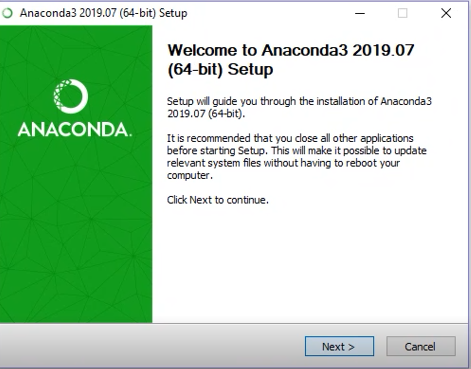
\includegraphics[scale=0.5]{figures/3}}
        \caption{Welcome to Anaconda Setup}
		\label{langkah2}
\end{figure}


\item Pada \textit{License Agreement} klik \textit{I Agree}
 gambar \textit{License Agreement}.

\begin{figure}[H]
    \centering
    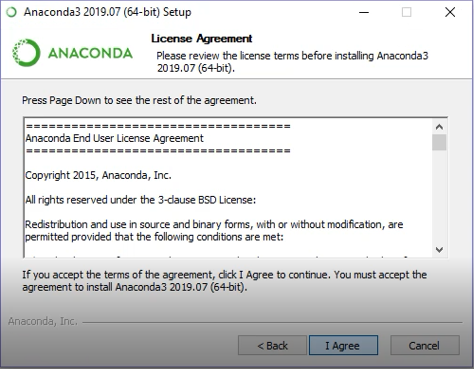
\includegraphics[scale=0.5]{figures/4}
    \caption{\textit{License Agreement}}
    \label{Figureanaconda3}
\end{figure}


\item Kemudian pilih \textit{Just Me(Recomended)} agar sesuai dengan komputer yang digunakan, kemudian klik \textit{next}
 gambar \textit{Just Me(recomended)}.

\begin{figure}[H]
    \centering
    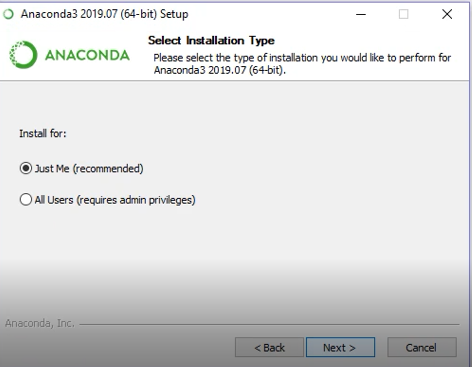
\includegraphics[scale=0.5]{figures/5}
    \caption{\textit{Just Me(recomended)}}
    \label{Figureanaconda4}
\end{figure}


\item Kemudian pilih lokasi tempat \textit{menginstall anaconda}
 gambar \textit{Pilih lokasi}.

\begin{figure}[H]
    \centering
    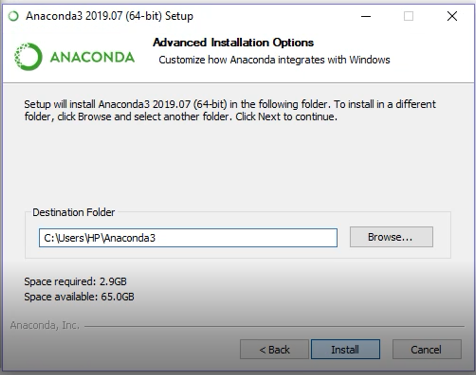
\includegraphics[scale=0.5]{figures/6}
    \caption{\textit{Pilih lokasi}}
    \label{Figureanaconda5}
\end{figure}

\item Kemudian centang \textit{Add Anaconda to my Path environtment variable}, agar saat \textit{menginstall selenium} langsung ke \textit{path anaconda} tidak ke aplikasi yang lain. Klik \textit{install}
 gambar \textit{Centang Anaconda to my PATH}.

\begin{figure}[H]
    \centering
    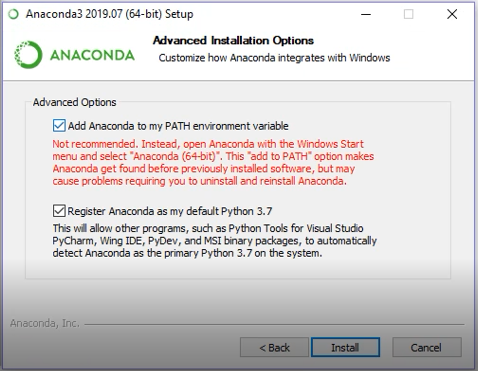
\includegraphics[scale=0.5]{figures/7}
    \caption{\textit{Centang Anaconda to my PATH}}
    \label{Figureanaconda6}
\end{figure}

\item Tunggu sampai proses \textit{installasi} selesai
 gambar \textit{Installation Complete}.

\begin{figure}[H]
    \centering
    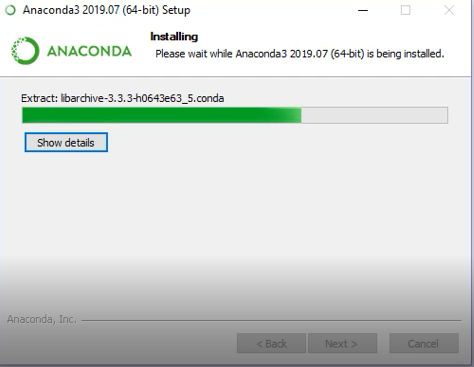
\includegraphics[scale=0.5]{figures/8}
    \caption{\textit{Installation Complete}}
    \label{Figureanaconda7}
\end{figure}

\item Apabila instalasi telah selesai klik \textit{next}
\begin{figure}[H]
    \centering
    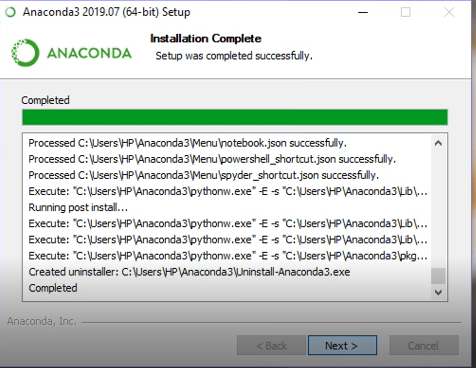
\includegraphics[scale=0.5]{figures/9}
    \caption{\textit{Installation Complete}}
    \label{Figureanaconda8}
\end{figure}

\item klik \textit{next}
\begin{figure}[H]
    \centering
    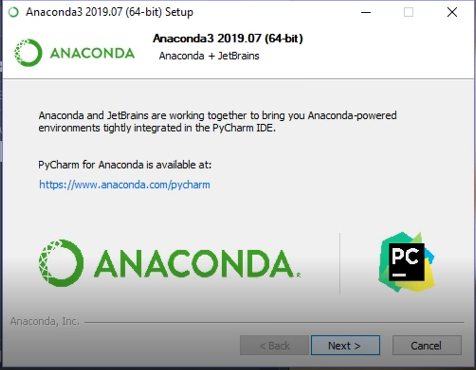
\includegraphics[scale=0.5]{figures/10}
    \caption{\textit{Anaconda+JetBrains}}
    \label{Figureanaconda70}
\end{figure}

\item Jika sudah klik \textit{finish}
 gambar \textit{Thanks fo install Anaconda}.

\begin{figure}[H]
    \centering
    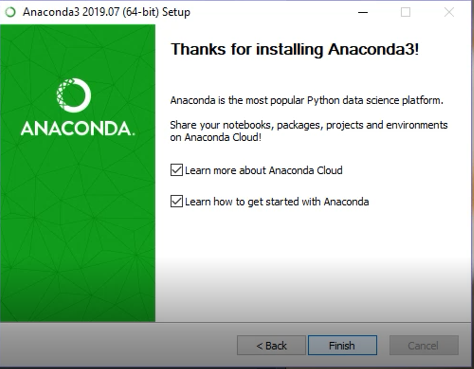
\includegraphics[scale=0.5]{figures/11}
    \caption{\textit{Thanks for install Anaconda}}
    \label{Figureanaconda70}
\end{figure}
\end{enumerate}

\section{Instalasi Pip}
\subsection{Windows (Windows 10)}
\begin{enumerate}
\item buka anaconda promt
\item ketikkan conda install -c anaconda pip
\begin{figure}[H]
    \centering
    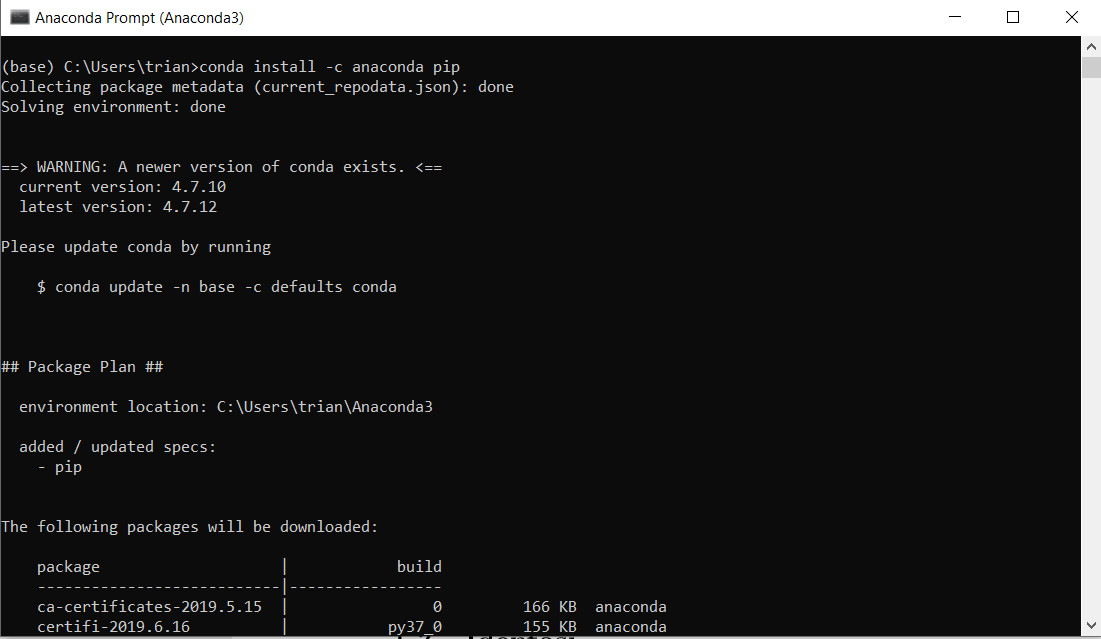
\includegraphics[scale=0.5]{figures/installpip (2)}
    \caption{\textit{Install pip}}
    \label{Figureanaconda70}
\end{figure}
\item ketik y, lalu enter. Tunggu hingga proses instalasi selesai.
\begin{figure}[H]
    \centering
    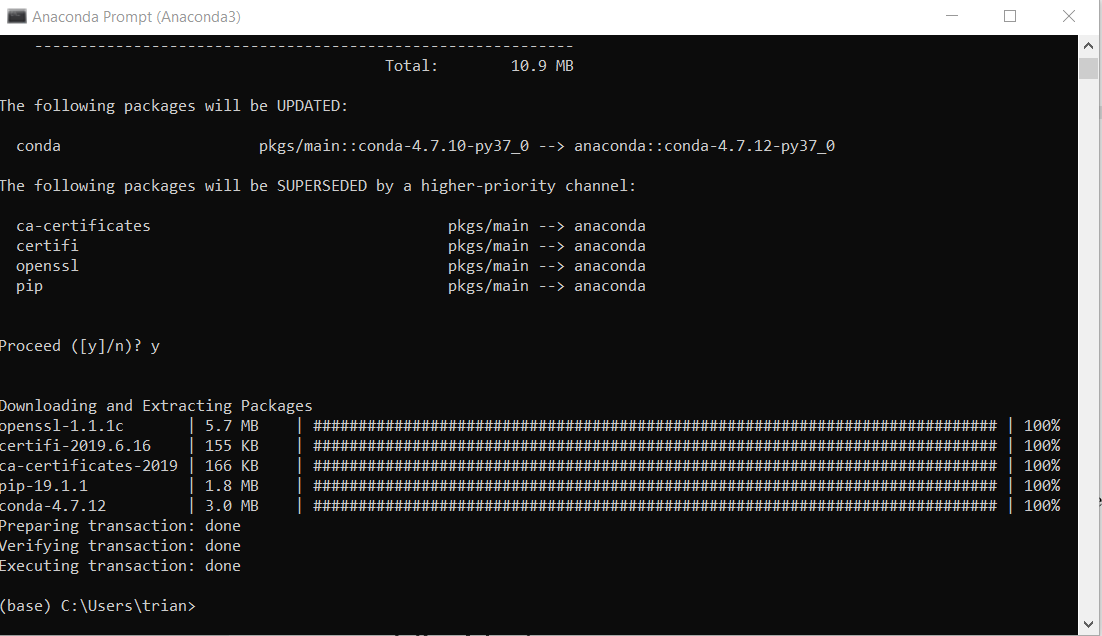
\includegraphics[scale=0.5]{figures/pipselesai}
    \caption{\textit{Install pip Selesai}}
    \label{Figureanaconda70}
\end{figure}
\item jika telah selesai, lakukan pengecekan versi pip dengan mengetikkan pip -V
\begin{figure}[H]
    \centering
    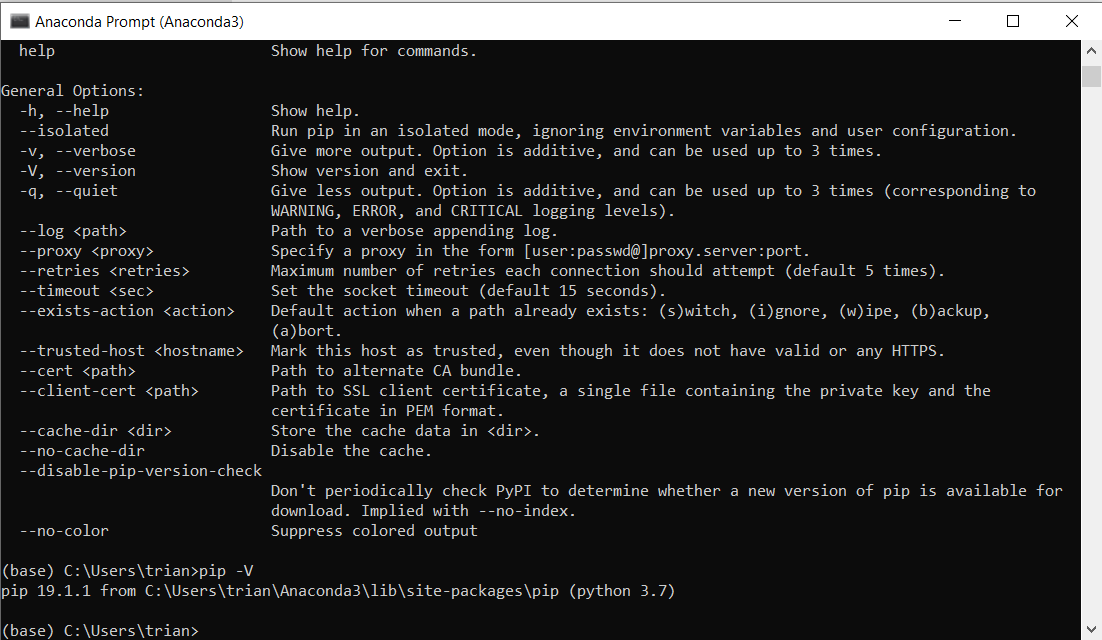
\includegraphics[scale=0.5]{figures/pipversion}
    \caption{\textit{Melihat Versi pip}}
    \label{Figureanaconda70}
\end{figure}

\end{enumerate}

\subsection{Linux (Ubuntu 19.04)}
\begin{enumerate}

\item pertama kita buka terminal kita lalu ketikkan perintah \textbf{sudo apt install python3-pip -y} untuk pip3 dan \textbf{sudo apt install python-pip -y} untuk pip contoh seperti gambar \ref{installpip}, lalu enter
\begin{figure}[H]
\centering
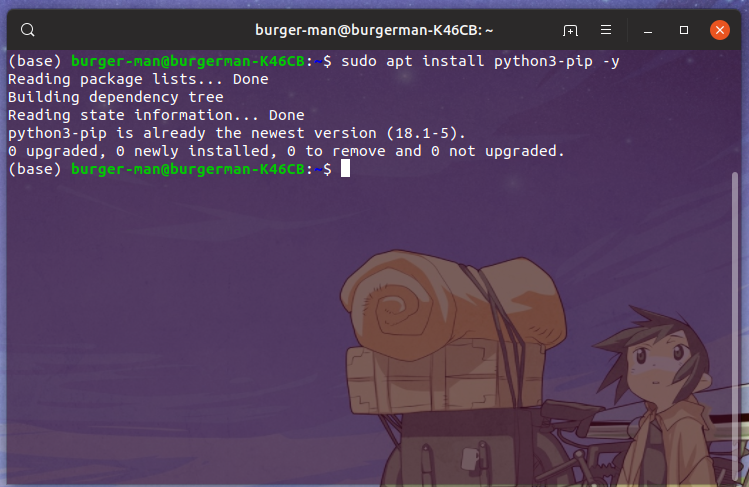
\includegraphics[width=1\textwidth]{figures/installpip.png}
\caption{Gambar instal pip}
\label{installpip}
\end{figure}

\end{enumerate}

\section{Setting Environment}
\subsection{Windows (Windows 10)}
\begin{enumerate}
\item Buka file explorer
\item Klik kanan pada This pc, lalu pilih properties
\begin{figure}[H]
    \centering
    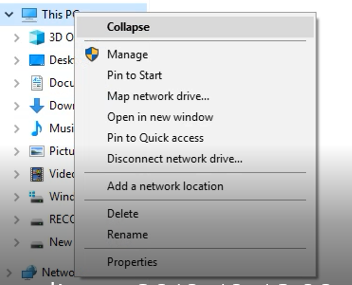
\includegraphics[scale=0.7]{figures/properties}
    \caption{\textit{Properties}}
    \label{Environment1}
\end{figure}
\item Pilih menu Advanced system settings
\begin{figure}[H]
    \centering
    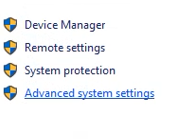
\includegraphics[scale=0.7]{figures/advanced}
    \caption{\textit{Advanced system settings}}
    \label{Environment2}
\end{figure}
\item Pilih Environment Variables
\begin{figure}[H]
    \centering
    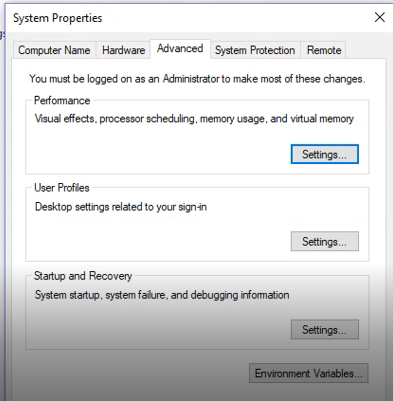
\includegraphics[scale=0.7]{figures/environment}
    \caption{\textit{Environment Variables}}
    \label{Environment3}
\end{figure}
\item Pilih Path
\begin{figure}[H]
    \centering
    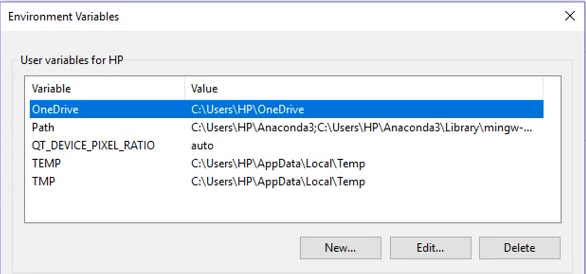
\includegraphics[scale=0.7]{figures/path}
    \caption{\textit{Path}}
    \label{Environment4}
\end{figure}
\item lalu pilih environment variable yang ingin ditambahkan, klik OK
\begin{figure}[H]
    \centering
    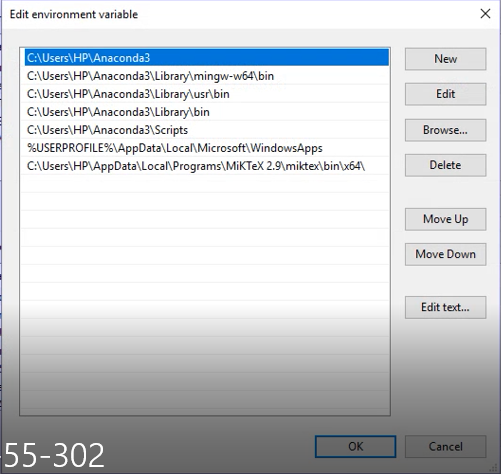
\includegraphics[scale=0.7]{figures/ok}
    \caption{\textit{Edit Environment Variable}}
    \label{Environment5}
\end{figure}
\end{enumerate}

\subsection{Linux (Ubuntu 19.04)}
\begin{enumerate}

\item pertama kita buka terminal kita lalu ketikkan perintah export PYTHONPATH=\$PYTHONPATH:pathinstallasipythonkalian contoh seperti gambar \ref{setpath}, lalu enter
\begin{figure}[H]
\centering
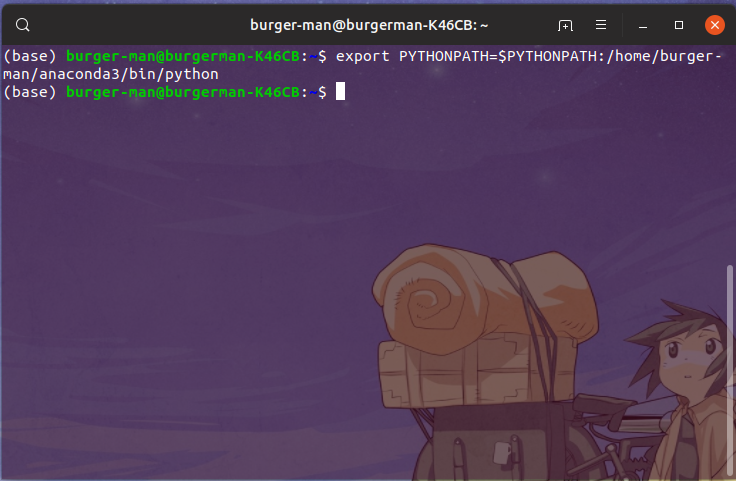
\includegraphics[width=1\textwidth]{figures/setpath.png}
\caption{Gambar setpath}
\label{setpath}
\end{figure}

\end{enumerate}

\section{Command Line Interface/Interpreter}
\subsection{Windows (Windows 10)}
\begin{enumerate}
\item Buka command prompt lalu ketikkan python
\item Buatlah perintah print, input, perkalian, dan pembagian
\item Bisa juga menjalankan file .py yang telah dibuat di IDE dengan cara python namafile.py, lalu klik enter
\begin{figure}[H]
    \centering
    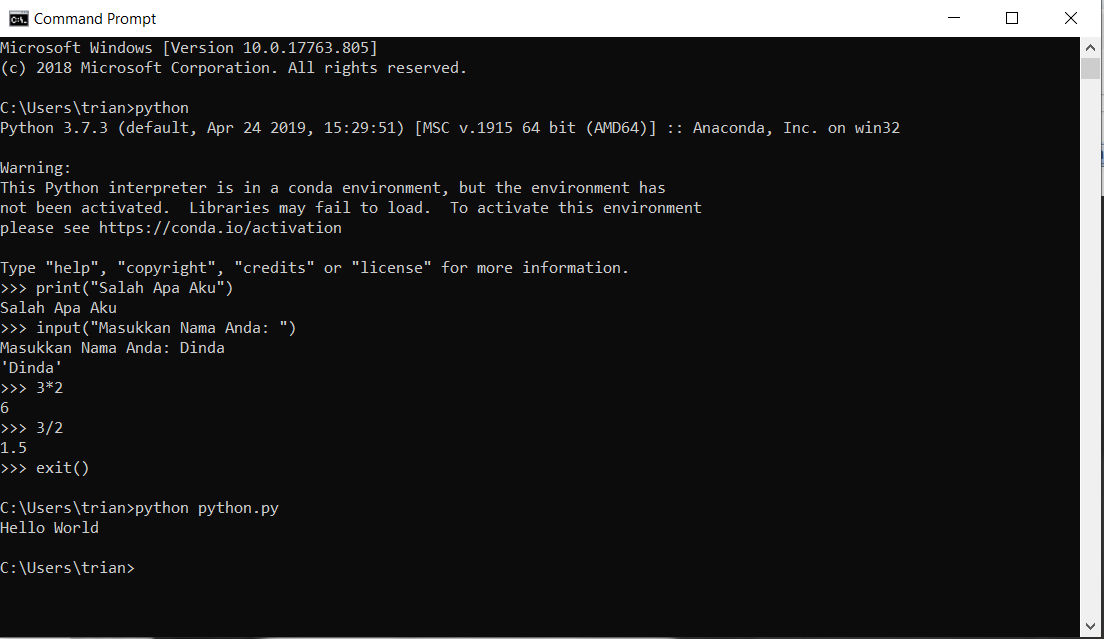
\includegraphics[scale=0.5]{figures/cli (2)}
    \caption{\textit{CLI in Command Prompt}}
    \label{CLI}
\end{figure}
\end{enumerate}

\subsection{Linux (Ubuntu 19.04)}
Untuk menjalankan perintah CLI cukup mudah yaitu sebagai berikut

\begin{enumerate}

\item Buka terminal lalu ketikkan \textbf{python \textit{namafile}.py} seperti gambar ~\ref{cli}, lalu enter
\begin{figure}[H]
\centering
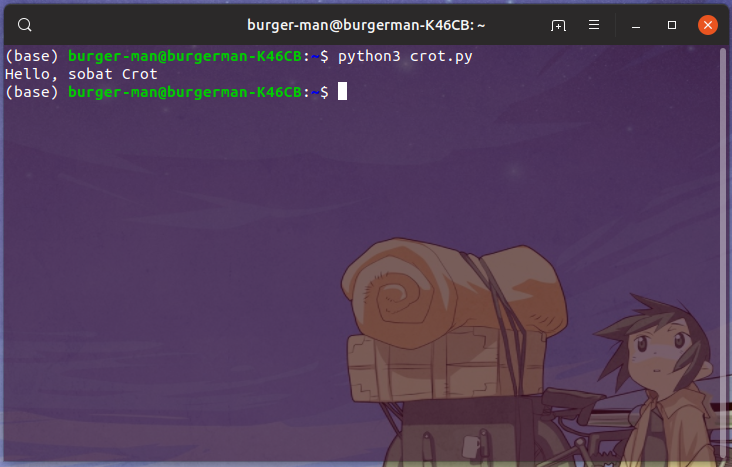
\includegraphics[width=1\textwidth]{figures/cli.png}
\caption{Gambar running script dengan CLI}
\label{cli}
\end{figure}

\end{enumerate}